\chapter{PROJECT PLAN}

\section{Project Timeline}

Figure~\ref{fig:timeline} presents the 10-week project timeline for the \textit{Probabilistic Path Optimization using Pruned Dijkstra} project. Tasks are organized in three overlapping phases: implementation (Weeks~1--4), testing and experimentation (Weeks~4--7), and analysis, writing, and presentation (Weeks~7--10). This phased structure ensures that correctness is validated before experimentation begins, and that experimental results directly inform the final report and presentation.

\begin{figure}[h!]
\centering
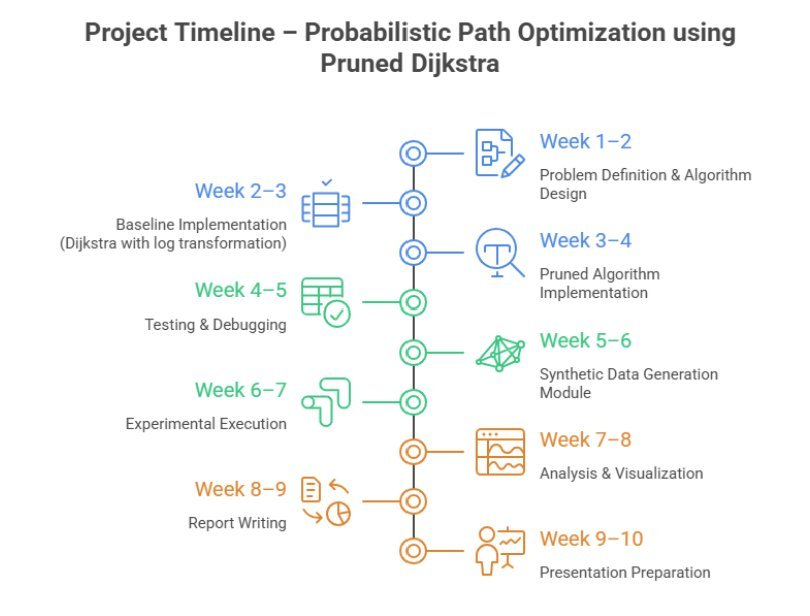
\includegraphics[width=0.85\textwidth]{timeline.png}
\caption[Project timeline]{Project timeline for \textit{Probabilistic Path Optimization using Pruned Dijkstra}. The timeline is structured across 10 weeks, alternating between left and right panels along a central spine. Blue entries correspond to the implementation phase (Weeks~1--4), green to the testing and experimentation phase (Weeks~4--7), and orange to the writing and presentation phase (Weeks~7--10). Each task overlaps with the subsequent one to allow iterative refinement.}
\label{fig:timeline}
\end{figure}

\section{Milestones}

The following milestones define the key delivery points of the project:

\begin{enumerate}
    \item \textbf{Core Implementation Completed:} End of Week~4\\
    Both the baseline Dijkstra algorithm and the probability-pruned Dijkstra algorithm will be fully implemented, tested on small hand-computed graphs, and validated for correctness against ground-truth optimal paths.

    \item \textbf{Experiments Completed:} End of Week~7\\
    All experimental runs across small, medium, and large graph configurations will be completed, with all metrics (execution time, peak memory, nodes explored, edges relaxed, optimality gap, MaxPQSize) recorded and verified.

    \item \textbf{Report Completed:} End of Week~9\\
    The full project report will be finalized, incorporating experimental results, visualizations, complexity validation, and the time--memory--optimality trade-off discussion.

    \item \textbf{Final Presentation Ready:} Week~10\\
    Presentation slides and a live demonstration of the implementation will be prepared for the final project presentation on 12~March~2026.
\end{enumerate}
